\only<1,2,3>{
\begin{tikzpicture}[remember picture,overlay]
    \node[anchor=north west, rotate=0, gray, font=\small] at (-1,-7.2) {
    [1] S. McAleer et al., Solving the rubik’s cube with approximate policy iteration
    };
\end{tikzpicture}
}


\begin{minipage}{0.62\textwidth}
\only<1>{
	Data annotation by  Bellman Equation:
	\begin{enumerate}
		\item $d(V_2) = d(V_0) + 1 = 1$
		\item $d(V_4) = d(V_2) + 1 = 2$
		\item $d(V_5) = d(V_4) + 1 = 3$
		\item $d(V_1) = d(V_5) + 1 = 4$ \\ $d(V_6) = d(V_5) + 1 = 4$
	\end{enumerate}
}
\only<2, 3>{
	Model $J(V)$ is trained to predict $d$. \vspace{5mm}

	Until convergence repeat:
    \begin{itemize}
        \iitem{for $V \in \text{dataset}$ calculate $J'(V)$}
        \iitem{train model to predict $J'(V)$}
    \end{itemize}
    \vspace{5mm}
    
    \only<3>{
	Important details:
    \begin{itemize}
        \iitem{dataset generation}
        \iitem{model architecture}
        \iitem{vertex representation}
        \iitem{model-based pathfinding}
    \end{itemize}
    }


}
\end{minipage}
\hfill
\begin{minipage}{0.36\textwidth}
Bellman equation: \vspace{-2mm}
\begin{equation*}
	\phantom{42} \hfill \boxed{J'(V) = 1 + \min_\sigma J(\sigma V)}
\end{equation*}
\vspace{-10mm}

\begin{figure}[h]
    \centering
    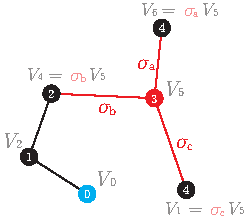
\includegraphics{imgs/pAsset 4.pdf}
    %\caption{}
    %\label{fig:}
\end{figure}


\end{minipage}

\only<2>{
\vfill 
Instead of storing a dictionary with all the vertices, we train the model to <<remember>>/<<understand>> the values found according to Bellman.
}